\documentclass[../../main.tex]{subfiles}

\begin{document}

    Category theory is the language needed to give simplicial/cyclic sets a simple definition. It is also an essential part of the language of algebraic topology. It begins with the elementary definitions of categories, functors, natural transformations and adjunctions.

    \begin{definition}
        A \defemph{category} is a collection of objects $ob(\cat{C})$ such that for every pair of objects $x, y \in ob(\cat{C})$ there is a collection $hom(x, y)$ of \defemph{arrows} or \defemph{morphisms} from $x$ to $y$. These are said to have $x$ as their \defemph{domain} and $y$ as \defemph{codomain}. If $f \in hom(A, B)$ it is often written $f: x \to y$ and $\domain{f} = x, \codomain{f} = y$.
        
        For all $x, y, z \in ob(\cat{C})$ there is a composition of arrows 
        
        \begin{align*}
            \circ: hom(x, y) \times hom(y, z) &\to hom(x, z) \\ 
            f, g &\mapsto g \circ f = gf
        \end{align*}
        
        that fulfills the following axioms.

        \begin{enumerate}
            \item Associativity: (fg)h = f(gh) for all arrows f,g,h where composition is defined
            \item Identity: For every $c \in ob(C)$ there is an arrow $\idarrow[c]: c \to c$ such that $f \circ id_C = f$ and $g \circ id_c = g$ for all arrows $f, g$ where this composition is defined.
        \end{enumerate}
    \end{definition}

    \begin{definition}
        If $hom(x, y)$ is a set for every choice of $x$ and $y$, $\cat{C}$ is \defemph{locally small}. If also $ob(\cat{C})$ is a set, \defemph{C} is \defemph{small}. 
    \end{definition}
    
    Every category $\cat{C}$ has an associated category $\cat{C^{op}}$ formed by reversing all arrows in $\cat{C}$. Every statement in $\cat{C}$ can be made in $\cat{C^{op}}$ and is then called the \defemph{dual} statement. Its truth value is invariant.

    \begin{example}
        An example of a category would be the category of topological spaces, usually denoted $\cat{Top}$, with objects being topological spaces and morphisms being continuous functions. Another example of a category would be $\cat{hTop}$ with the same objects but homotopy equivalence classes as morphisms. Yet another category would be $\cat{Haus}$ where instead the objects are topological spaces with the Hausdorff property and continuous functions as morphisms.
    \end{example}

    \begin{definition}
        A (\defemph{covariant}) \defemph{functor} $\functor{F}: \cat{C} \to \cat{D}$ consists of a map of objects in $\cat{C}$ to objects in $\cat{D}$ and one map of morphisms in C to morphisms in D such that the following is fulfilled for all objects $a, b, c$ and arrows $g: a \to b, f: b \to c$.
        
        \begin{enumerate}
            \item $\domain{\functor{F}(f)} = \functor{F}(b), \codomain{\functor{F}(f)} = \functor{F}(c)$ \label{covar1}
            \item $\functor{F}(\idarrow[c]) = \idarrow[\functor{F}(c)]$
            \item $\functor{F}(fg) = \functor{F}(f) \circ \functor{F}(g)$ \label{covar2}
        \end{enumerate}
    \end{definition}

    If \ref{covar1} and \ref{covar2} are reversed to
    
    \begin{enumerate}
        \item [\ref{covar1}*.] $\domain{\functor{F}(f)} = \functor{F}(c), \codomain{\functor{F}(f)} = \functor{F}(b)$ \label{cov1}
        \item [\ref{covar2}*.] $\functor{F}(fg) = \functor{F}(g) \circ \functor{F}(f)$ \label{cov2}
    \end{enumerate}

    , $\functor{F}$ is instead \defemph{contravariant}. The contravariance/covariance in conjunction with the duality of categories can be somewhat disorienting. One can interchange a contravariant functor from a category, $\cat{C}$, to a covariant from the opposite, $\cat{C^{op}}$.

    \begin{example}\label{functor_exmp}
        A few examples of functors include:
        \begin{itemize}
            \item the forgetful functor $G$, which forgets structure, e.g. taking a group to its underlying set and group homomorphisms to their underlying function
            \item $\mathcal{P}$ is a functor which maps a set to its power set and functions $f:X\to Y$ to the map which sends $V\subseteq X $ to $f(V)\subseteq Y$. 
            \item if B and C are categories then a diagram of shape B in C is a covariant functor $D:B\to C$
        \end{itemize}
    \end{example}

    These examples are illustrative and are but a small fraction of functors. The forgetful functor is a general notion, simply leaving out or "forgetting" structure can be done in many cases. The last example stated above might seem roundabout and will be properly treated next. 
    
    Inside a given category $\cat{C}$, we often study some small, often finite, part of it. This is called a \defemph{diagram} in $\cat{C}$. Formally, an $\cat{I}$-shaped diagram $\functor{D}$ in $\cat{C}$ is a functor $\functor{D}: \cat{I} \to \cat{C}$, where $\cat{I}$ is called an \emph{index category}. If $\cat{I}$ is small, $\functor{D}$ is called a small diagram. Diagrams are a central concept in relation with them commuting. A \defemph{commutative diagram} is defined such that all directed paths with identical start and end points lead to the same results by composition. More exactly $|hom_I(A,B)|\leq 1$, there is at most one morphism between any objects $A,\,B$. Commutative diagrams play the role in category theory that equations play in algebra (see Barr–Wells, Section 1.7).%check quote 
    
    If to a diagram $\functor{D}$ in $\cat{C}$, we add an object $e$ and arrows from $e$ to each object in $\functor{D}$ such that the resulting new diagram commutes, $e$ and the arrows form a \defemph{cone} over $\functor{D}$. A cone that is universal, in the sense that every other cone factors through it uniquely, is called a \defemph{limit} over $\functor{D}$. When a limit exist, it might not be unique. However, any other limit will be isomorphic to it. The dual notions are \defemph{cocones} and colimits. Important examples of limits are products are products, pullbacks, equalizers and terminal objects.
    
    \begin{figure}[H]
        \centering
        \begin{subfigure}[b]{0.5\textwidth}
            \centering
            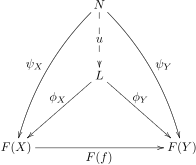
\includegraphics[scale=.65]{Functor_cone}
            \caption{}
        \end{subfigure}%
        ~ 
        \begin{subfigure}[b]{0.5\textwidth}
            \centering
            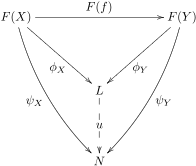
\includegraphics[scale=.65]{Functor_co-cone}
            \caption{}
        \end{subfigure}
        \caption{The cone/co-cone (left, right respectively) $(N,\Psi)$ factors/cofactors through the cone $(L,\phi)$ uniquely with $u$, the latter cone $(L,\phi)$ is then denoted the limit/colimit.}
    \end{figure}
    
    The categorical \defemph{product} can be easily defined in terms of limits. 
    
    \begin{definition}
        Given objects $\{c_i\}_{i \in I}$ in $\cat{C}$, their \defemph{product} is a limit over the diagram containing all $c_i$ and no arrows other than their identities.
    \end{definition}
    
    Examples of products is the cartesian product in $\cat{Set}$, the topological product in $\cat{Top}$ and the direct product in $\cat{Grp}$. In these categories, any set of objects has a product with these explicit constructions. The main reason of having the topological product defined the way it is(finitely many $O_i \neq X_i$) is to make it the categorical product in $\cat{Top}$. Would we not have this requirement(also known as the \emph{box topology} on $X$) it would merely be a cone over the discrete diagram of all $c_i$.
    
    As usual, there is a dual concept to products called a coproduct. Reverse all arrows in the definition of a product and one has a coproduct
    
    \begin{figure}[H]
        \centering
        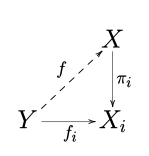
\includegraphics[scale=.7]{Cat_product}
        \caption{Diagram of a product. \textit{If Y is some object and for every i in I, $\pi_i:Y\to X_i$ is a morphism, then there exists a unique map $f:Y\to X$ such that for each i in I the diagram commutes.}}
        \label{fig:product}
    \end{figure}

    Examples of coproducts is the disjoint union in $\cat{Set}$ as well as its sibling, the disjoint union of topological spaces in $\cat{Top}$. This means that the cartesian product of topological spaces and the disjoint union of topological spaces are dual constructions. The same goes in $\cat{Set}$.

    For two functors $\functor{A}, \functor{B}$ with the same target one can define the \defemph{comma category} $(\functor{A} \downarrow \functor{B})$, which is read "$\functor{A}$ comma $\functor{B}$". This concept is needed to give a categorical description of the \textit{geometric realization} of simplicial sets.

    \begin{definition}
        Given functors $\functor{A}: A \to C$, $\functor{B}: B \to C$, the category $(\functor{A} \downarrow \functor{B})$ has its objects made up up triplets $(a, b, f)$ where $a \in A$, $b \in B$ and $f \in hom(\functor{A}(a), \functor{B}(b))$ and arrows between $(a, b, f)$ and $(a', b', f')$ made up of commutative diagrams of the following type.
    \end{definition}

    \begin{figure}[H]
        \[
            \begin{tikzcd}
                \functor{A}(a) \arrow[r, "f"] \arrow[d, "\functor{A}(\phi)"]
                & \functor{B}(b) \arrow[d, "\functor{B}(\psi)"] \\
                \functor{A}(a') \arrow[r, "f'"]
                & \functor{B}(b')
            \end{tikzcd}
        \]
    \end{figure}
    
    One of the most important concepts in category theory is adjunctions. According to Saunders MacLane: \textit{“Adjoint functors arise everywhere.”}\cite{cate-mac}.
    
    \begin{definition}
        Given $\functor{F}: \cat{D} \to \cat{C}$ and $\functor{G}: \cat{C} \to \cat{D}$, $\functor{F}$ is called \defemph{left adjoint} to $\functor{G}$ if for every $X \in C, Y \in D$ there is a bijection of hom-sets, $$\cat{C}(\functor{F}Y, X) \cong \cat{D}(Y, \functor{G}X)$$, which is natural in both $Y$ and $X$. $\functor{G}$ is then \defemph{right adjoint} to $\functor{F}$.
    \end{definition}
    
    An example of adjunctions are letting $\functor{G}$ be the forgetful functor mapping $\cat{Grp} \to \cat{Set}$. Its left adjoint is then $\functor{F}: \cat{Set} \to \cat{Grp}$ which sends a set $A$ to the free group on $A$. The bijections arise from the fact that a group homomorphism is completely described by its action on the generators.
    
    Another example is the abelianization functor $\functor{F}: \cat{Grp} \to \cat{Ab}$. It is left adjoint to the forgetful functor $\functor{G}: \cat{Ab} \to \cat{Grp}$. This is due to the fact that the commutator subgroup $[G, G]$ of any group $G$ needs to lie in the kernel of any homomorphism into an abelian group. This means that any such homomorphism will factor uniquely through the projection $G$ onto $G^{ab}$.
    
    For every set $X$, there are two canonical ways of defining a topology on it, the trivial topology and the discrete topology. These are in fact functors $\functor{F}: \cat{Set} \to \cat{Top}$. Assigning the discrete topology to $X$ by $\functor{F}$ will mean that any map \emph{from} it is continuous. Therefore we have a bijection between functions from $X$ into a given topological space $Y$ and continuous maps between $X$ and $Y$. This means that this functor is left adjoint to the forgetful functor $\functor{G}: \cat{Top} \to \cat{Set}$. If instead we let $\functor{F}$ assign the trivial topology to $X$, every function \emph{to} $X$ is continuous and by the opposite argument $\functor{F}$ is right adjoint to $\functor{G}$.
    
    The \emph{Yoneda lemma} is perhaps the most important result in elementary category theory. It tells us something essential about representable functors which will be defined. In every category $\cat{C}$ and $A \in \cat{C}$ there is a covariant functor $h^A: \cat{C} \to \cat{Set}$, often denoted $\mathrm{Hom}_\cat{C}(A, -)$. It sends objects $X \mapsto \mathrm{Hom}_\cat{C}(A, X)$ and arrows $f \mapsto f \circ -$. In fact, 
    
    \begin{equation*}
        h^-: 
        \begin{cases}
            A \mapsto h^A \\
            f \mapsto f \circ -
        \end{cases}
    \end{equation*}
    
    is a contravariant functor called the \emph{Yoneda embedding}, $h^-: \cat{C}^{op} \to \cat{Set}^\cat{C}$.
    
    \begin{definition}
        A functor $\functor{F}: \cat{C} \to \cat{Set}$ is called \defemph{representable} if there is an object $A \in \cat{C}$ such that there is a natural isomorphism $h^A \cong \functor{F}$.
    \end{definition}
    
    \begin{theorem}[Yoneda lemma]
        Any functor $\functor{F}: \cat{C} \to \cat{Set}$ has a bijection for all $A \in C$ 
        $$\functor{F}(A) \cong \mathrm{Nat}(h^A, \functor{F})$$ 
        natural in $A$.
    \end{theorem}
    
    \begin{proof}
        Consider the following diagram of a natural transformation $\Phi$ between $h^A$ and $\functor{F}$ applied to $A$ and an arbitrary object $X \in C$. 
        
        \begin{figure}[H]
            \centering
            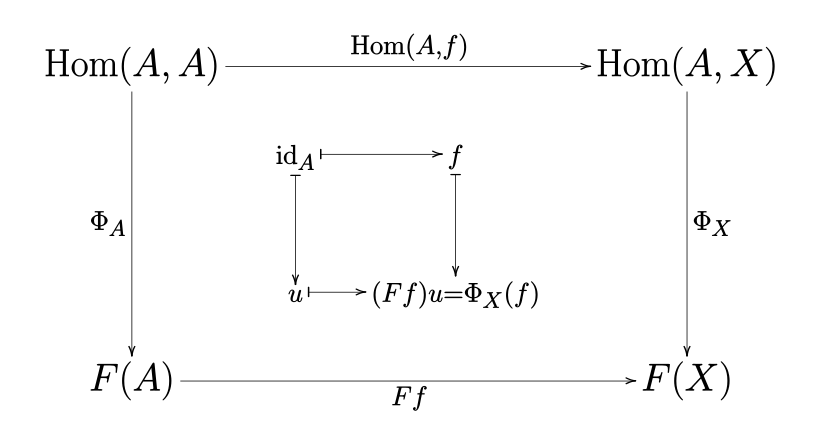
\includegraphics[scale=.35]{Yoneda_lemma_c}
            \caption{Diagram of natural transformation}
            \label{fig:boat1}
        \end{figure}

        Let $u$ be the action of $\Phi_A$ on $\idarrow[A]$. By looking at both ways of sending $\idarrow[A]$ to $\functor{F}(X)$ it is realized that the action of $\Phi_X$ on any $f \in \mathrm{Hom}(A, X)$ is given by 

        \begin{equation}
            \Phi_X(f) = \functor{F}f(u)
        \end{equation}
        
        This means that $\Phi$ is completely determined by its action on the identity which can take on any value in $\functor{F}(A)$.
    \end{proof}

\end{document}